\chapter{Unifying Benchmark Review Frameworks with MESA}
\label{ch:mesa}

\todo[inline]{Integrate the full content, tables, and verified statistics from \texttt{MESA-meta-evaluation-standard-for-ai/mesa\_paper.tex} (\texttt{main} branch). Cross-reference Appendix~\ref{app:mesa_rubric} for the complete concern list and 39-criterion rubric.}

\section{Sorting 280 Framework Items into 30 Shared Concerns}
\label{sec:mesa_concerns}

\todo[inline]{Detail the mapping of 280 questions across BetterBench~\cite{reuel_betterbench}, ECBD~\cite{liu_ecbd_2024}, Scorecard~\cite{san_joaquin_scorecard_2026}, How2Bench~\cite{cao_how2bench_2025}, Agentic Benchmark Checklist~\cite{zhu_agentic_benchmark_checklist_2025}, Benchmark Caliper~\cite{corona_benchmark_caliper_2026}, and OECD facets~\cite{cohn_hernandez_orallo_oecd_2023} onto 30 shared concerns, plus recoding rules into favorable, unfavorable, and unresolved outcomes.}

\section{The 39-Criterion MESA Rubric}
\label{sec:mesa_rubric}

\todo[inline]{Present the derived 39-criterion \mesa{} rubric separating descriptive benchmark metadata from evaluative evidence judgments, and separating six source-support levels from check outcomes.}

\section{Empirical Study Design}
\label{sec:mesa_design}

Figure~\ref{fig:mesa_overview} summarizes the two-study empirical design evaluating existing frameworks and the derived \mesa{} rubric across four benchmarks: HumanEval~\cite{chen_codex_humaneval_2021,human_eval_repository}, TruthfulQA~\cite{lin_truthfulqa_2022,truthfulqa_repository}, Humanity's Last Exam~\cite{phan_etal_hle_2025}, and $\tau$-bench~\cite{tau_bench_repository}.

\begin{figure}[htbp]
    \centering
    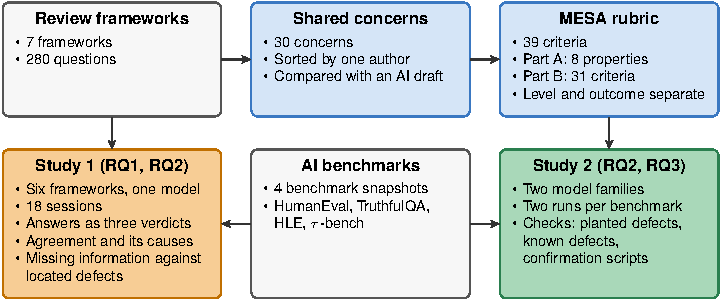
\includegraphics[width=\textwidth]{Figures/mesa_study_overview.pdf}
    \caption{Overview of the MESA two-study empirical design: Study~1 compares six existing review frameworks on four benchmarks, and Study~2 evaluates the 39-criterion MESA rubric across two reviewer model families (Claude and Gemini) using repeatability, planted-defect, and known-defect checks.}
    \label{fig:mesa_overview}
\end{figure}

\subsection{Study 1: Six Frameworks on Four Benchmarks}
\label{sec:mesa_study1_design}

\todo[inline]{Describe Study~1 execution protocol, frozen paper and repository snapshots, read-only tool boundaries, comparison against framework authors' earlier assessments (125 matched items), and disagreement coding.}

\subsection{Study 2: Two Model Families and Three Verification Checks}
\label{sec:mesa_study2_design}

\todo[inline]{Describe Study~2: two model families (Claude and Gemini) applying the 39-criterion rubric twice per benchmark, plus planted-defect fixtures, seven known real benchmark defects, and script-based verification.}

\section{Results}
\label{sec:mesa_results}

\subsection{Framework Agreement (RQ1)}
\label{sec:mesa_rq1}

\todo[inline]{Import verified Study~1 agreement tables: six frameworks agreed on 159 of 302 comparisons (159 of 252 excluding 50 question-scope differences) and matched framework authors' verdicts on 93 of 125 items (70 exact answers).}

\subsection{Missing Information versus Located Defects (RQ2)}
\label{sec:mesa_rq2}

\todo[inline]{Import verified Study~1 missing-information analysis: 210 answers penalized missing information compared with 13 citing an actual located defect.}

\subsection{Rubric Repeatability and Defect Detection (RQ3)}
\label{sec:mesa_rq3}

\todo[inline]{Import verified Study~2 results: Claude and Gemini agreed on 88\% to 91\% of verdicts and 61\% of the six evidence levels; both detected every planted defect; of seven known real defects, Gemini failed the matching criterion for one or two per run, and confirmation scripts verified all 14 failed ratings.}

\section{Worked Case and Implications for Requirements Engineering}
\label{sec:mesa_worked_case}

\todo[inline]{Include the worked benchmark-rating case from \texttt{mesa\_paper.tex} and transition into Chapter~\ref{ch:decisions}, showing how a structured \mesa{} review record becomes an input to requirement admissibility rules.}
